De lijsten met events kunnen behoorlijk lang zijn in Event Viewer. Het zou makkelijker zijn als we alleen de belangrijke events kunnen zien, bijvoorbeeld alleen Critical en Error. En gelukkig kan dat ook in Event Viewer.

\begin{minipage}[t]{\linewidth}
\raggedright
\adjustbox{valign=t}{%
	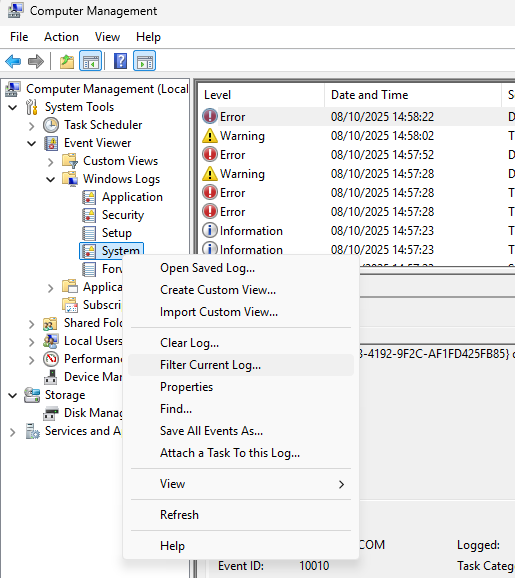
\includegraphics[width=0.99\linewidth]{ev-filter.png}%
}
\end{minipage}

Door rechts te klikken op het logboek kan je \textquote{Filter Current Log...} selecteren. In het nieuwe venster is het mogelijk om te filteren op Event level.

